\documentclass[border=0.8ex,svgnames,tikz]{standalone}
\usepackage{amsmath,mathtools}
\usepackage{fontspec}
\setmainfont{Source Serif 4}
\setsansfont{Source Sans 3}
\setmonofont{Source Code Pro}

\usetikzlibrary{positioning,calc}

\begin{document}
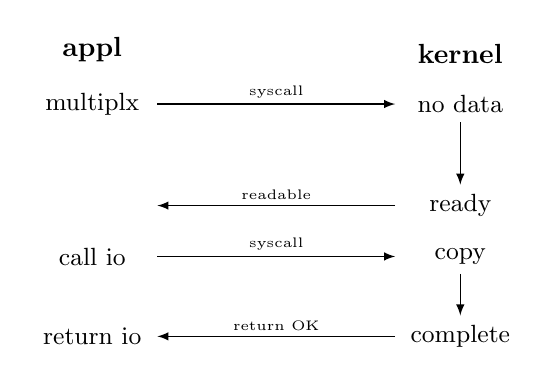
\begin{tikzpicture}
  \coordinate(appl) at (0,0);
  \coordinate(kernel) at ($(appl)+(13.3em,0)$);
  \begin{scope}[
    every node/.style={
      align=center,
      anchor=center,
      font=\small,
      text width=4em,
    },
    ]
    \node                          (noready)  {no data};
    \node[below=2.25em of noready] (ready)    {ready};
    \node[below=0.45em of ready]   (copy)     {copy};
    \node[below=1.50em of copy]    (complete) {complete};
  \end{scope}
  \begin{scope}[
    every node/.style={
      align=center,
      anchor=center,
      font=\small,
      text width=4em,
    },
    ]
    \node (multiplxing) at ($(noready)-(kernel)-(appl)$)       {multiplx};
    \node (return1)     at ($(multiplxing)+(ready)-(noready)$) {};
    \node (call-io)     at ($(copy)-(kernel)-(appl)$)          {call io};
    \node (return2)     at ($(call-io)+(complete)-(copy)$)     {return io};
  \end{scope}
  \begin{scope}[
    every node/.style={above,font=\tiny,inner sep=0.45ex},
    every path/.style={draw,>=latex},
    ]
    \path[->]
    (multiplxing) edge node{syscall}   (noready)
    (noready)     edge                 (ready)
    (ready)       edge node{readable}  (return1)
    (call-io)     edge node{syscall}   (copy)
    (copy)        edge                 (complete)
    (complete)    edge node{return OK} (return2);
  \end{scope}
  \node[above=1ex of multiplxing]{\bfseries appl};
  \node[above=1ex of noready]{\bfseries kernel};
\end{tikzpicture}
\end{document}
